Now the protocol presented in \cite{giordani2020} which utilises quantum walk dynamics in order to generate higher dimensional entanglement is summarised.

The imagined setup of this protocol is that there are two labs, $A$ and $B$, which have a shared source of entangled qubits but are otherwise spatially separated and cannot interact with one another.

In this section we use following notation:
\begin{itemize}
    \item $\ket{\psi}_J$ is a state belonging to the subspace $\mathcal{H}_J = \mathcal{H}^{(A)}_J \otimes \mathcal{H}^{(B)}_J, J\in\{C,W\}$.
    \item $\ket{\psi}^{(K)}$ is a state belonging to the subspace $\mathcal{H}^{(K)} = \mathcal{H}^{(K)}_C \otimes \mathcal{H}^{(K)}_W, K\in\{A,B\}$.
    \item  $\ket{\psi}^{(K)}_J$ is a state belonging to the subspace $\mathcal{H}^{(K)}_J$.
\end{itemize}

In this mathematical framework the overall Hilbert space is comprised of two quantum walk subspaces,
\begin{align}
    \mathcal{H} &= \mathcal{H}^{(A)} \otimes \mathcal{H}^{(B)}\\
                &= \mathcal{H}^{(A)}_C \otimes \mathcal{H}^{(A)}_W \otimes \mathcal{H}^{(B)}_C \otimes \mathcal{H}^{(B)}_W.
\end{align}

The basic premise of this protocol is this:
\begin{enumerate}
    \item Entangle the two coin spaces of the walkers $\mathcal{H}^{(K)}_C$. (Fig \ref{fig:preparation}.)
    \item Proceed with the quantum walk for some determined number of steps.
    \item Use a projective measurement $\mathcal{P}_\gamma = \ket{\gamma}\bra{\gamma}, \ket{\gamma}\in\mathcal{H}^{(A)}_C$ to then transfer the entanglement so that it solely exists in the subspace $\mathcal{H}^{(A)}_W \otimes \mathcal{H}^{(B)}_C \otimes \mathcal{H}^{(B)}_W$.
    \item In similar fashion, find a projection $\mathcal{P}_\delta = \ket{\delta}\bra{\delta}, \ket{\delta}\in\mathcal{H}^{(B)}_C$ to transfer the entanglement to exist between the two walker subspaces, $\mathcal{H}^{(i)}_W$, only.
    \item Accumulate entanglement in the walker subspaces by once more entangling the two coin spaces and repeating the protocol.
\end{enumerate}

\begin{figure}
    \centering
    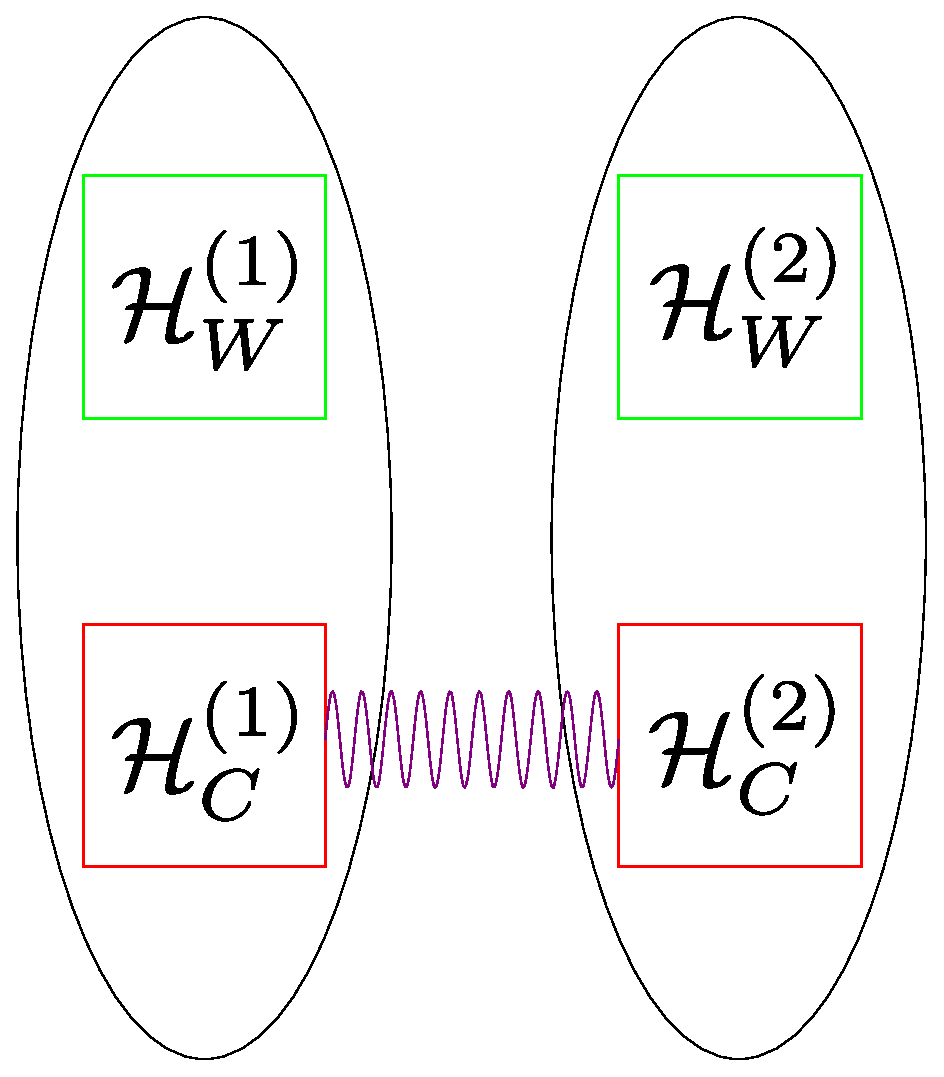
\includegraphics[scale = .25]{preparation}
    \caption{The initial prepared state has entanglement solely between the two coin subspaces. Figure is an edited version of FIG 3 from \cite{giordani2020}.}
    \label{fig:preparation}
\end{figure}

In this way, arbitrary amounts of higher dimensional entanglement can be generated.
The ordering of steps 3 and 4 is not overly important since the full operators describing the projective measurements are given by
\begin{align}
    \ket{\gamma}\bra{\gamma} \otimes I \otimes I \otimes I\\
    I \otimes I \otimes \ket{\delta}\bra{\delta} \otimes I
\end{align}
which clearly commute.
As is the case with many quantum walk based protocols, particular attention must be paid to the choice of coin used for the quantum walk, as it will have a large impact on the outcomes of the protocol.
The shift operator used in this protocol is the $\tilde{S}$, as outlined in section \ref{subsubsection:q_r_w}.

\subsection{Transfer using identity coin operator}
\label{subsection:qw_transfer}
To illustrate the basic principles of the protocol, consider the case where our coin is the identity $I$.
\begin{enumerate}
    \item A state $\ket{\psi(0)}$ is prepared with the coin states entangled and walkers at the origin
    \begin{equation}
        \ket{\psi(0)} = \underbrace{\frac{1}{\sqrt{2}}\Big [\ket{\uparrow}^{(A)}_C\ket{\uparrow}^{(B)}_C + \ket{\downarrow}^{(A)}_C\ket{\downarrow}^{(B)}_C \Big]}_{\text{Bell State}}\otimes \ket{0}^{(A)}_W\ket{0}^{(B)}_W.
    \end{equation}
    \item The "coin", $I$, is applied and followed by the shift operator $\tilde{S}$ to advance the quantum walk.
    Explicitly (dropping the indices and combining some of our kets together) the walk evolves to the state
    \begin{equation}
        \ket{\psi(1)} = \tilde{S}I\ket{\psi} = \frac{1}{\sqrt{2}}\Big [\ket{\uparrow,\uparrow}\ket{0,0} + \ket{\downarrow,\downarrow}\ket{1,1}\Big].
    \end{equation}
    \item Using the operator $\mathcal{P}_{\gamma} = \ket{\gamma}\bra{\gamma}$ the part of $\ket{\psi(1)}$ residing in the $\mathcal{H}^{(A)}_C$ subspace is projected onto the state $\ket{\gamma}$. \newline
    For this example, choose $\ket{\gamma} = \frac{1}{\sqrt{2}} \big [\ket{\uparrow} + \ket{\downarrow} \big]$ which then gives
    \begin{equation}
        \mathcal{P}_\gamma \ket{\psi(1)} = \frac{1}{2}\Big [\ket{\gamma}\otimes \big (\ket{\uparrow, 0, 0} + \ket{\downarrow, 1, 1}\big )\Big ].
    \end{equation}
    \item Similarly, project the other coin onto $\ket{\delta}$ which in this instance is taken to be the same state as $\ket{\gamma} = \frac{1}{\sqrt{2}} \big [\ket{\uparrow} + \ket{\downarrow} \big]$,
    \begin{equation}
        \mathcal{P}_\delta \mathcal{P}_\gamma \ket{\psi(1)} = \frac{1}{2\sqrt{2}}\Big [\ket{\gamma}\otimes \ket{\delta} \otimes \frac{1}{\sqrt{2}}\Big (\ket{0, 0} + \ket{1, 1}\Big )\Big ].
    \end{equation}
\end{enumerate}
Renormalising gives the final state
\begin{equation}
    \label{equation:qw_transfer_1_final}
    \ket{\gamma}^{(A)}_C \otimes \ket{\delta}^{(B)}_C \otimes \underbrace{\frac{1}{\sqrt{2}}\Big [\ket{0, 0} + \ket{1, 1}\Big ]_W}_{\text{Bell State}},
\end{equation}
which has a Bell state in the $\mathcal{H}_W$ subspace, and the states in $\mathcal{H}_C$ are separable.
Therefore the entanglement that originally resided in the coin subspace has been transferred to the walker one.

\subsection{Accumulation}
\label{subsection:qw_accumulation}
The true motivation behind this protocol is the ability to accumulate the entanglement transferred from the lower dimensional coin subspace to the higher dimensional walker one.
This is done by repeating the entire process with some small changes.
Again $I$ is used as the coin.
\begin{enumerate}

    \item Starting with the final state obtained from the first iteration of the protocol (equation \ref{equation:qw_transfer_1_final}) the coin subspaces are re-entangled, obtaining a new initial state $\ket{\psi(0)}$,
    \begin{alignat}{3}
        \ket{\gamma}^{(A)}_C \otimes \ket{\delta}^{(B)}_C&\otimes \frac{1}{\sqrt{2}}\Big [\ket{0, 0} + \ket{1, 1}\Big ]_W\\
        \overset{\text{Entangle }\mathcal{H}_C}{\longrightarrow} \frac{1}{\sqrt{2}} \Big [\ket{\uparrow, \uparrow} + \ket{\downarrow, \downarrow}\Big ]_C&\otimes \frac{1}{\sqrt{2}}\Big [\ket{0, 0} + \ket{1, 1}\Big ]_W\\
        & &:=\ket{\psi(0)}.
    \end{alignat}
    \item Now take two steps instead of one in the walk.
    \begin{align}
        \ket{\psi(2)} &= (\tilde{S}I)^2\ket{\psi(0)}\\
        &= \frac{1}{2}\Big[\ket{\uparrow,\uparrow}\big (\ket{0,0}+\ket{1,1}\big ) + \ket{\downarrow,\downarrow}\big (\ket{2,2} + \ket{3,3}\big )\Big ].
    \end{align}
    \itemrange{1} Using the same projection operators in the two coin subspaces, $\mathcal{P}_\gamma \in \mathcal{H}^{(A)}_C,  \mathcal{P}_\delta \in \mathcal{H}^{(B)}_C$, and renormalising gives the final state
    \begin{equation}
        \ket{\gamma}\otimes\ket{\delta}\otimes\frac{1}{2}\Big[\ket{0,0} + \ket{1,1} + \ket{2,2} + \ket{3,3}\Big ].
    \end{equation}
\end{enumerate}

Using claim \ref{claim:maximally_entangled_states}, the log negativity of
\begin{equation}
    \frac{1}{2}\Big[\ket{0,0} + \ket{1,1} + \ket{2,2} + \ket{3,3}\Big ]
\end{equation}
is 2, setting $d=4$ (since both of the qudits only have 4 states of non-zero amplitude they can be simulated by ququarts even if their their true dimension is greater than 4).
Therefore, 2 units of log negativity have been transferred from the Bell states (each of log negativity 1) to the qudit pair and optimal transfer has been achieved.
The process can be repeated to accumulate arbitrarily large amounts of entanglement into our walker subspace.
The number of steps needed in the quantum walk for each iteration is as follows.
\begin{claim}
\label{claim:min_steps}
The $n^{th}$ iteration (counting from 1) of the protocol requires at least $2^{n-1}$ steps in the quantum walk.
\end{claim}
\begin{proof}
Each step in a quantum walk with shift operator $\tilde{S}$ increases the number of basis states with non-zero amplitude by 1, provided that the amplitude $\ket{\downarrow}$ coin basis state is non-zero.
Therefore the dimension of each walker can be taken to be $s + 1$, where $s$ is the total number of steps taken in the walk, since the walker space can be reduced to the subspace spanned by the $s+1$ non-zero amplitude basis states.
Using Claim \ref{claim:maximally_entangled_states}, the upper bound on the entanglement that can be held between the two walker states is given by $\log_2(s+1)$ ebits.
This implies the following condition on the total number of steps
\begin{equation}
    \log_2(s+1) \geq n \implies s\geq 2^n -1.
\end{equation}
Assuming that this inequality is satisfied at equality for the $n-1^{th}$ iteration of the protocol gives a total step number of $2^{n-1} -1$.
Therefore, the minimum number of steps for the $n^{th}$ iteration is given by
\begin{align}
    2^{n} - 1 - (2^{n-1} -1) &= 2^n - 2^{n-1}\\
    &= 2 \times 2^{n-1} - 2^{n-1}\\
    &= 2^{n-1}.
\end{align}
\end{proof}
Whilst this is effective for the identity coin, for the general coin optimal transfer is not nearly as effective.
For example, when using the Hadamard coin, it is not possible to transfer all the entanglement to the qudits and instead they only become non-maximally entangled.

\subsection{Retrieval}
\label{subsection:qw_retrieval}
Although accumulating the entanglement in higher dimensions is of significant use, it is also possible to imagine that retrieving the entanglement back into the qubits would also be of use.
For example, consider the case where the method of generating entangled qubits is not deterministic but an algorithm requiring large numbers of Bell states is to be executed.
If the accumulation of entanglement can be reversed to get Bell pairs back, then the entangled Bell pairs can be stored in the qudits when they are successfully generated and then retrieved all at once to ensure the algorithm can be performed.
In the identity coin example, it is rather simple to use a near identical setup, where the qudits play the role of the coins and the qubits are the walkers, to retrive entangled Bell pairs out of the qudits.
For a general coin, it is also possible in principle to retrieve some entanglement back out of the entangled qudits.
However, retrieval after more than 1 ebit has been transferred for the non-identity coin is not simple within the framework of a quantum walk based protocol, due to the non maximal nature of the entanglement present in the qudits.
For example, figure \ref{fig:2ebittransfer} shows the maximal possible entanglement that can be transferred when the QW protocol is done twice using two Bell states is approximately 1.585, using the same projective operator $\mathcal{P}_\gamma$ on both of the coins.
*****Numerical simulations using different projective operators $\mathcal{P}_\gamma, \mathcal{P}_\delta$ show 1.585 is still the maximum possible.********
\begin{figure}
    \centering
    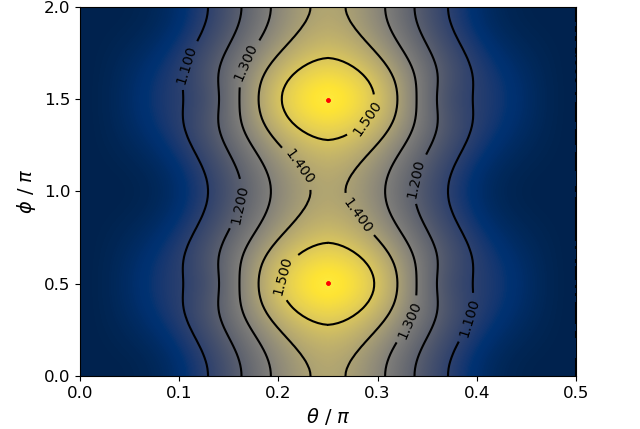
\includegraphics[scale=0.75]{2ebit_transfer.png}
    \caption{Transferring two ebits using the quantum walk protocol proposed by \cite{giordani2020}. $\theta, \phi$ are the parameters describing $\ket{\gamma}$ that defines the projection operator $\mathcal{P}_\gamma$.}
    \label{fig:2ebittransfer}
\end{figure}